\documentclass{article}
\usepackage[hmargin=1in,vmargin=1.5in]{geometry}
\usepackage{amsmath}
\usepackage{amsfonts}
\usepackage{graphicx}
\usepackage{subcaption}
\usepackage{bm}
\newcommand{\A}{\bm A}
\newcommand{\x}{\bm x}
\newcommand{\y}{\bm y}
\newcommand{\z}{\bm z}
\renewcommand{\a}{\bm a}
\renewcommand{\b}{\bm b}
\renewcommand{\c}{\bm c}
\renewcommand{\d}{\bm d}
\renewcommand{\v}{\bm v}
\newcommand{\p}{\bm p}
\newcommand{\q}{\bm q}
\newcommand{\1}{\bm 1}
\title{Homework 3}
\setcounter{MaxMatrixCols}{20}
\author{Xinyi Gu, Songchen Tan}
\date{\today}
\begin{document}
\maketitle
\section{}

\subsection*{(a)}
Let's arrange the arcs in the order $(1, 3), (2, 1), (2, 5), (3, 2), (3, 6), (4, 1), (5, 4), (6, 8), (7, 4), (7, 6), (8, 5), (8, 7)$. The incidence matrix is

$$
\begin{bmatrix}
+1&-1&0&0&0&-1&0&0&0&0&0&0\\
0&1&1&-1& 0&0&0&0& 0&0&0&0\\
-1&0&0&1& 1&0&0&0& 0&0&0&0\\
0&0&0&0& 0&1&-1&0& -1&0&0&0\\
0&0&-1&0& 0&0&1&0& 0&0&-1&0\\
0&0&0&0& -1&0&0&1& 0&-1&0&0\\
0&0&0&0& -1&0&0&1& 1&1&0&-1\\
0&0&0&0& 0&0&0&-1& 0&0&1&1
\end{bmatrix}
$$

\subsection*{(b)}

Please see the solution in Fig 1.

\begin{figure}
    \centering
    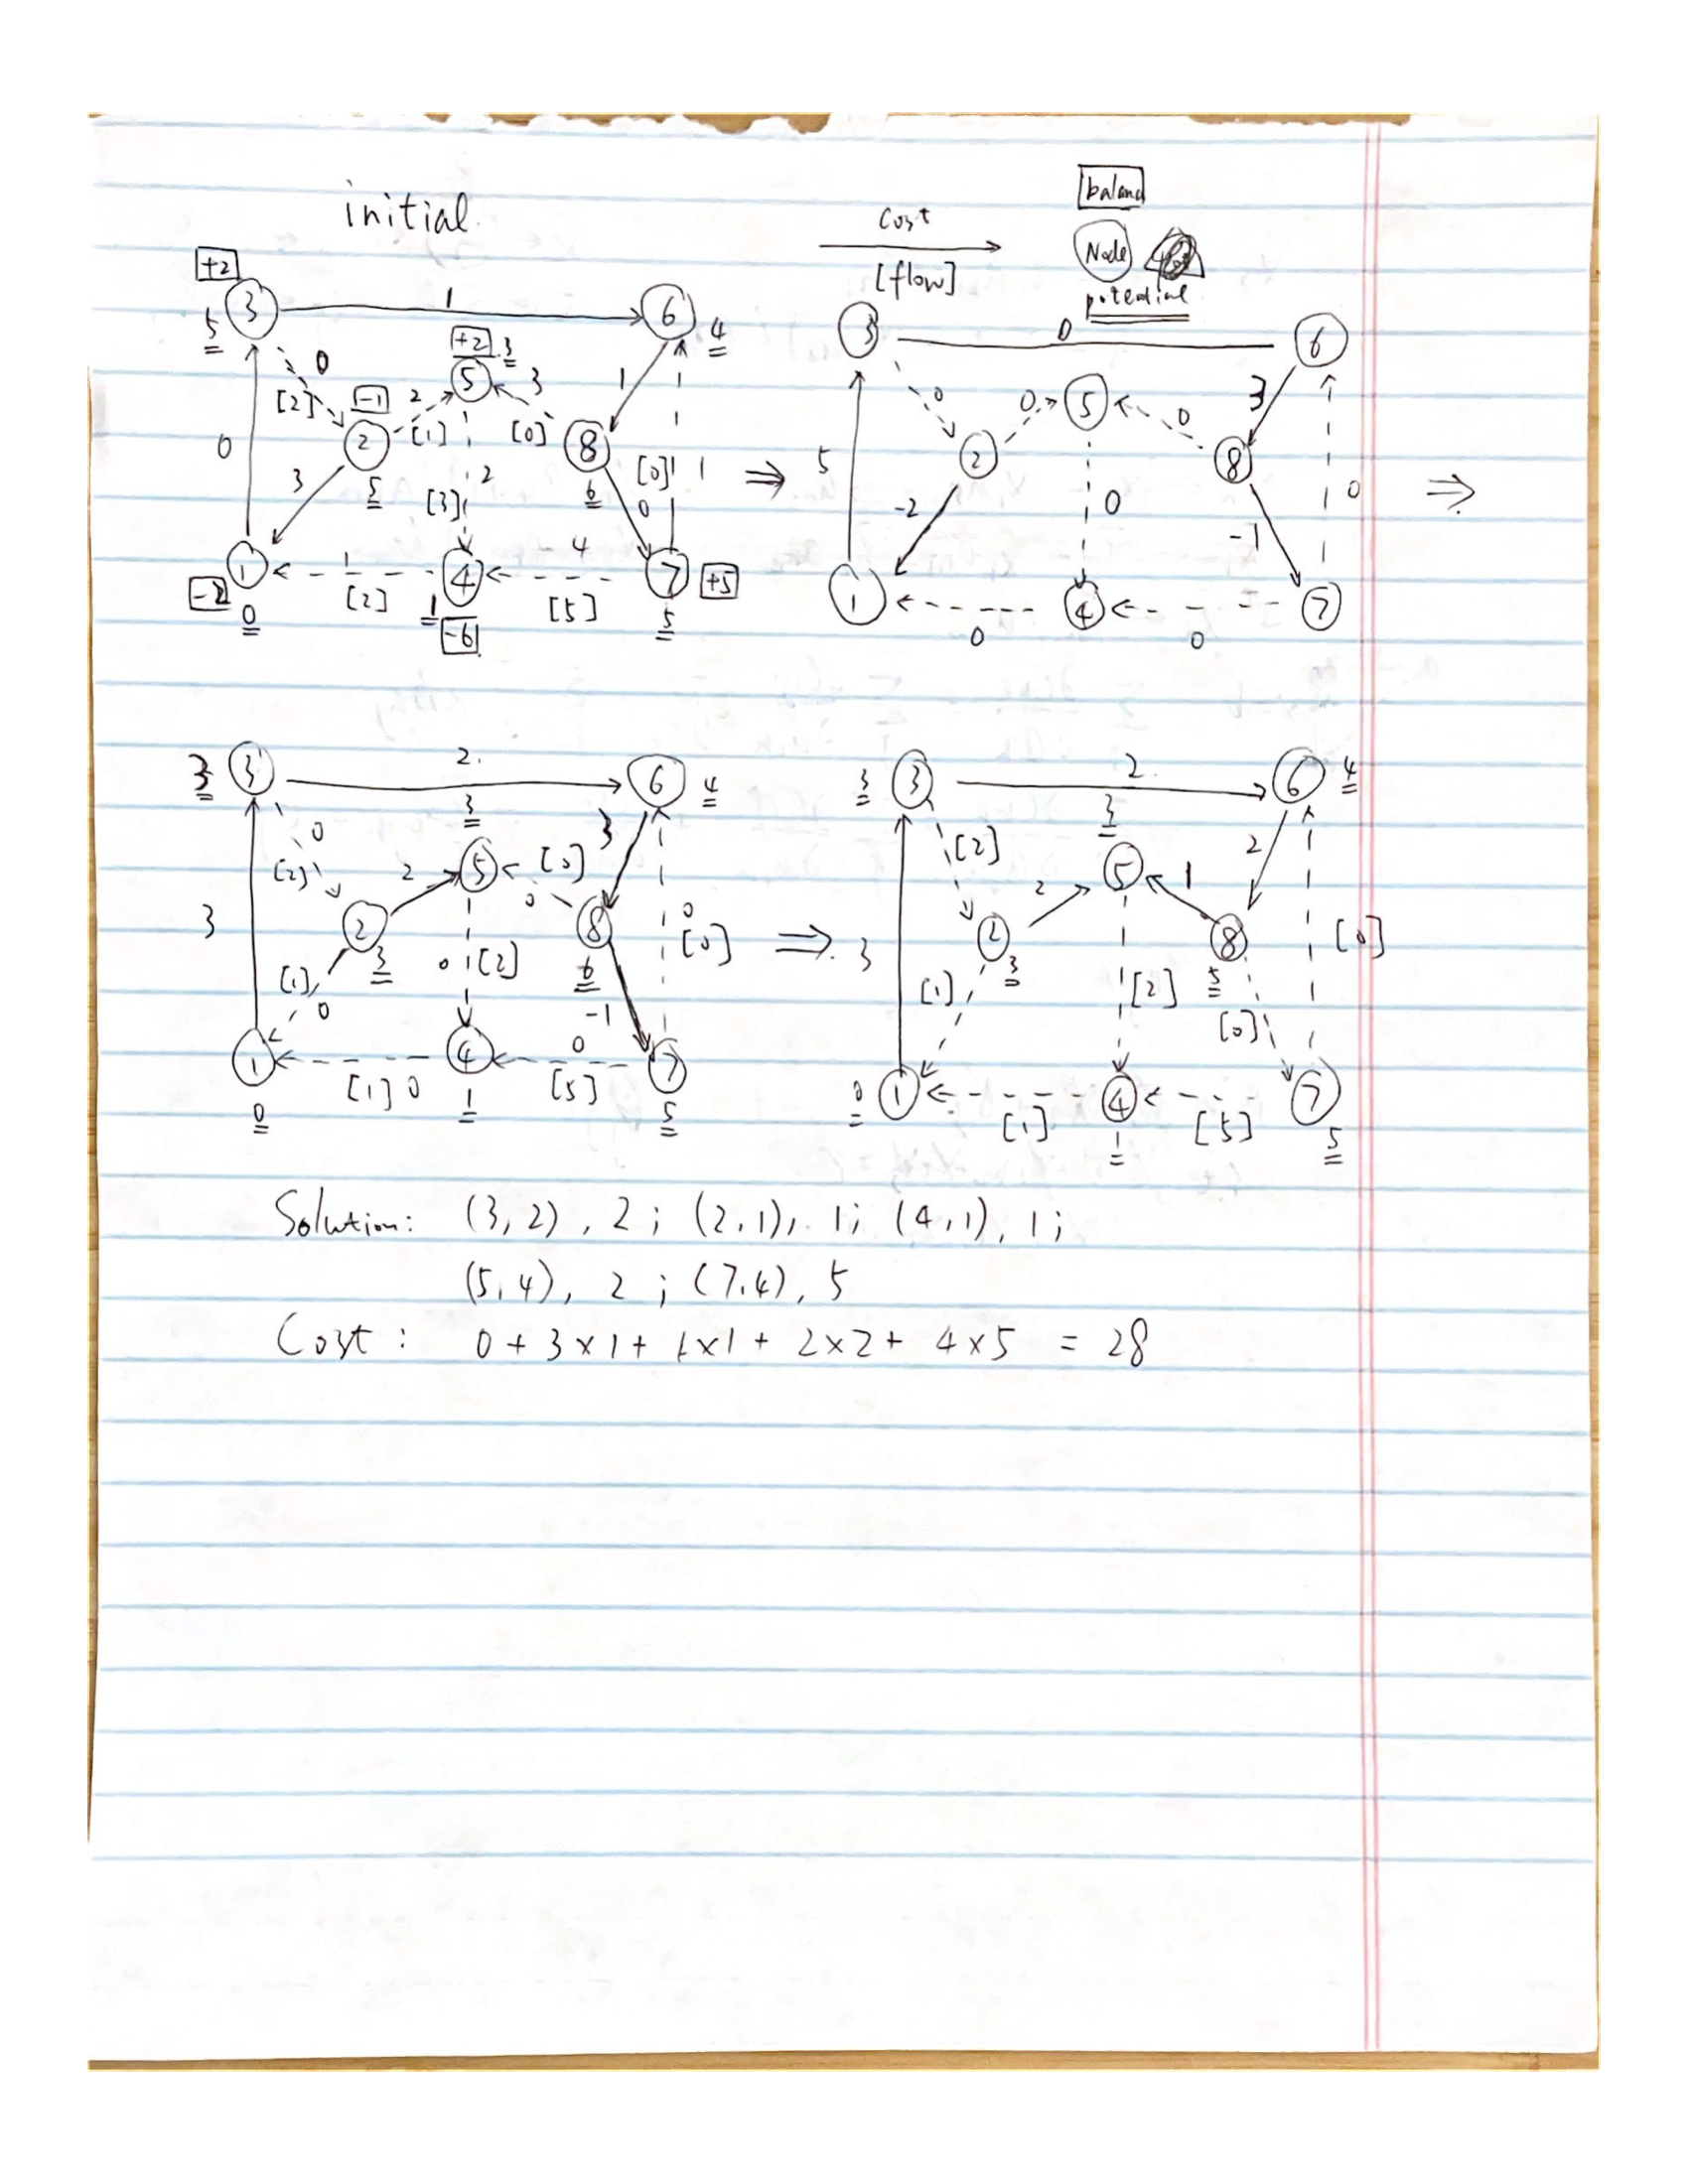
\includegraphics[width=\textwidth]{1.png}
    \caption{Solution to the Network Optimization Problem}
\end{figure}

\section{}

Considering $z$ as optimization variables, we can use $\max (a+Pz)^Tx=x^Ta+\max x^TPz$, subject to $z\in U$ where $U$ is defined as $Kz\le k$. The the dual problem would be $\min q^Tk$, subject to $q\ge0$ and $q^TK=x^TP$. Applying this formation to different sets:

\subsection*{(a)}

The set is represented by $z_i\le\rho,-z_i\le\rho,z=1,\cdots,p$. We introduce $2p$ variables $q_1,\cdots,q_{2p}$,

$$
\begin{aligned}
    \displaystyle
\rho\sum_iq_i&\le b-a^Tx\\
q_{2i-1}-q_{2i}&=\sum_j x_jP_{ji}\quad i=1,\cdots,p\\
q_i&\ge0\quad i=1,\cdots,2p
\end{aligned}
$$

\subsection*{(b)}

We introduce $m$ variables $q_1,\cdots,q_m$,

$$
\begin{aligned}
\displaystyle
q^Td&\le b-a^Tx\\
q^TD&=x^TP\\
q&\ge0
\end{aligned}
$$

\subsection*{(c)}

The set is represented by $2^p$ constraints, i.e. $\sum_i b_iz_i\le\rho$ where $b_i=\pm1$. We denote the matrix defined by $2^n$ constraints to be $D\in\mathbb R^{2^p\times p}$. We introduce $2^p$ variables $q_1,\cdots,q_{2^p}$ corresponding to them,

$$
\begin{aligned}
\displaystyle
\rho\sum_iq_i&\le b-a^Tx\\
q^TD&=x^TP\\
q&\ge0
\end{aligned}
$$

\section{}

We define two sets of variables: $s_{ij}$ to model the incidence between box $i$ and item $j$; $t_i$ to model the incidence between box $i$ and truck. The problem is formulated as $z=\min \sum_it_ib_i$, subject to

$$
\begin{aligned}
\displaystyle
\sum_is_{ij}&=1\quad\forall j\\
\sum_js_{ij}a_j&\le b_i\quad\forall i\\
(t_i&\ge s_{ij}\quad\forall j)\quad\forall i
\end{aligned}
$$

The move is possible in one travel only when $z\le Q$.

\section{}
\subsection{}
\begin{align*}
    \min \quad & x_1 + x_2 + x_3  \\
    \text{s.t.} \quad & x_1 + 2x_2+5x_3 = C \\
    & x_1, x_2, x_3 \in \mathbb{Z}^{n}_+
\end{align*}

Integer constraints can't be relaxed. Example:

Constraint relaxed formulation:

\begin{align*}
    \min \quad & x_1 + x_2 + x_3  \\
    \text{s.t.} \quad & x_1 + 2x_2+5x_3 = C \\
    & x_1, x_2, x_3 \geq 0
\end{align*}

$x = (1,1,2)^T$ is an optimal solution when $C = 13$ for the formulation with integer constraints. The optimal solution can be achieved when we use the 3rd kinds of coin only, if the integer constraints are relaxed, eg. $x = (0,0,2.6)^T$.

\subsection{}
\begin{align*}
    \max \quad & \sum^{n}_{i=1}\sum^{n}_{j=1} c_{ij}x_{ij}   \\
    \text{s.t.} \quad & \sum^{n}_{j=1} x_{ij} = 1, & i = 1, ..., n \\
    & \sum^{n}_{i=1} x_{ij} = 1, & j = 1, ..., n\\
    & x_{ij} \in \{0, 1\}
\end{align*}

Relaxed constraints:
\begin{align*}
    \min \quad & \sum^{n}_{i=1}\sum^{n}_{j=1} -c_{ij}x_{ij}   \\
    \text{s.t.} \quad & \sum^{n}_{j=1} x_{ij} = 1, & i = 1, ..., n \\
    & \sum^{n}_{i=1} x_{ij} = 1, & j = 1, ..., n\\
    & x_{ij} \geq 0 & \forall i,j
\end{align*}

The relaxed constraints formulation becomes an assignment problem. 
(a), $x_{ij} \leq 1$ is implised by constraints we have.
(b), by corollary 7.2, the assignment problem always has an integer optimal solution, i.e., in such problems when optimal cost is finite, all supplies are equal to 1 in this problem which is an integer, there exists and integer optimal flow vector.
$(a), (b) \Rightarrow x_{ij} \in \{0, 1\}$ 

\section{}

We define a source node $s$ and sink node $t$, together with one node for each team $p_i$ and one node for each pair $q_{ij}$. The edges $(s,q_{ij})$ have capacity $k$, edges $(q_{ij},p_i)$ and $(q_{ij},p_j)$ have capacity $k$, and edges $(p_j,t)$ have capacity $x_j$. There is a way to generate such a configuration $(x_1, \cdots,x_n)$ if and only if there is a flow saturating $t$.

\end{document}
